\documentclass[tikz,border=15pt]{standalone}
\usepackage{tikz}
\usetikzlibrary{positioning,shapes,arrows.meta,calc,fit,backgrounds,shadows}

\begin{document}
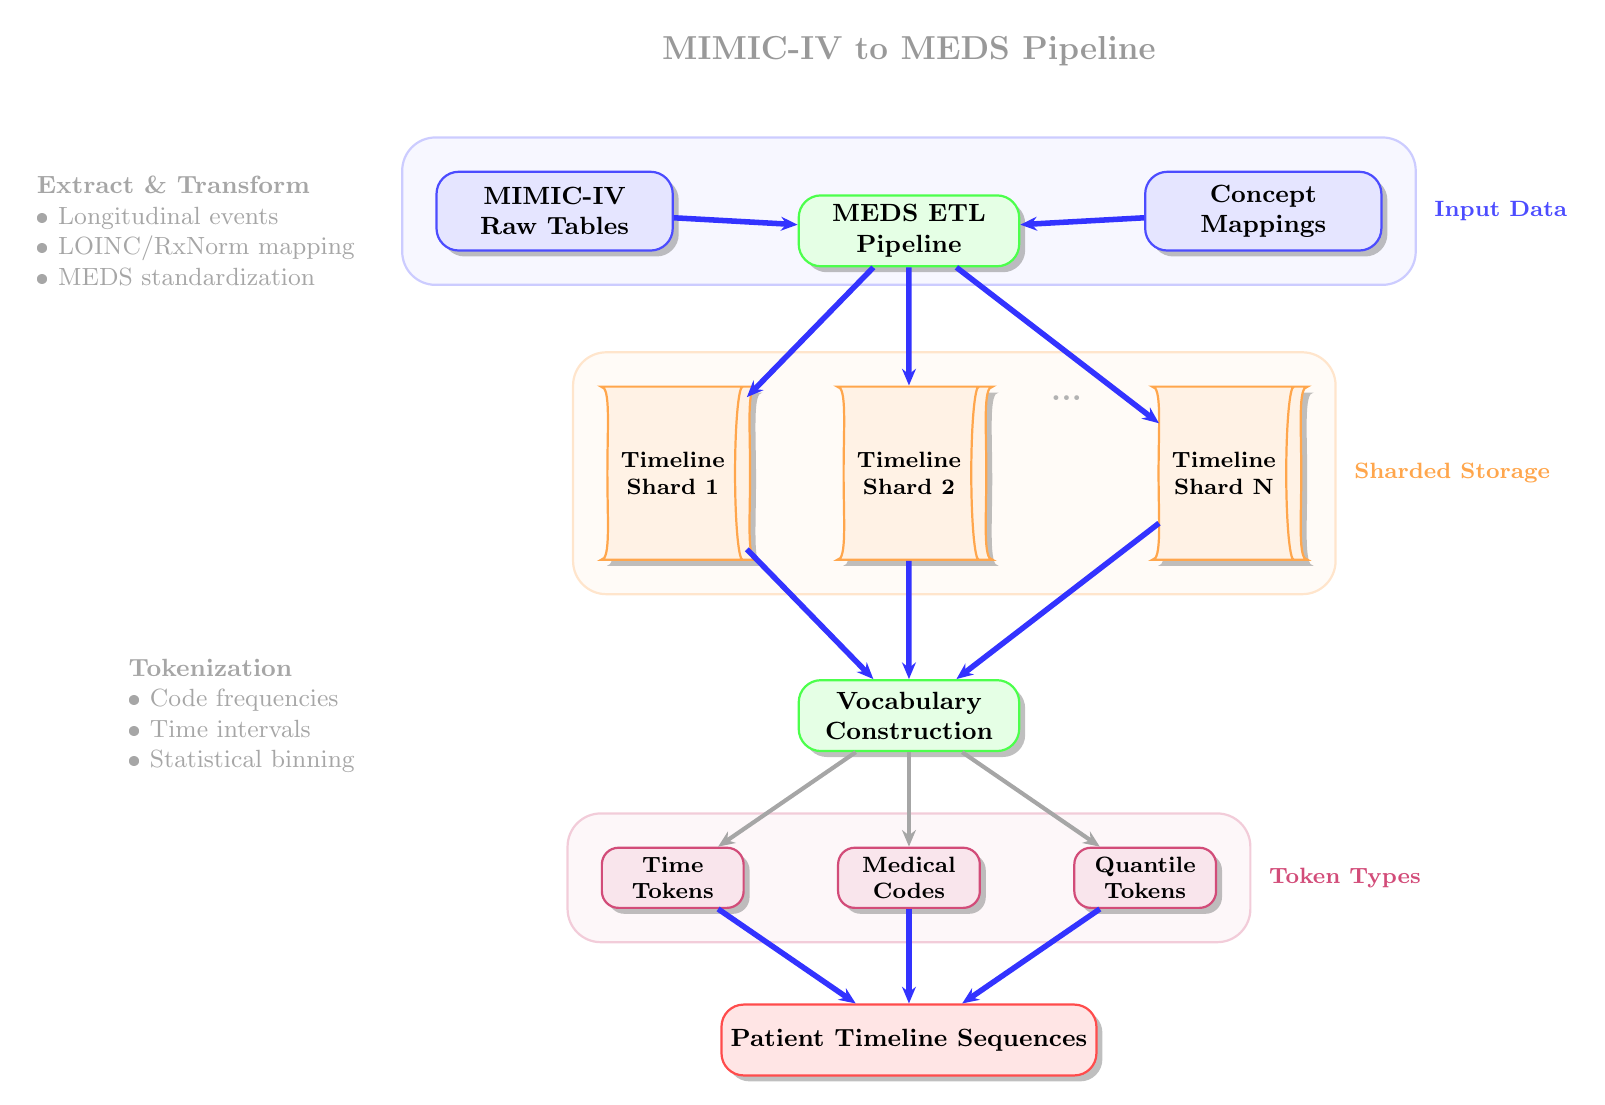
\begin{tikzpicture}[
    % Modern, clean styles
    data_source/.style={rectangle, draw=blue!70, fill=blue!10, rounded corners=8pt,
                       minimum width=3cm, minimum height=1cm, align=center,
                       font=\small\bfseries, thick, drop shadow},
    process_box/.style={rectangle, draw=green!70, fill=green!10, rounded corners=8pt, 
                       minimum width=2.8cm, minimum height=0.9cm, align=center, 
                       font=\small\bfseries, thick, drop shadow},
    storage/.style={cylinder, draw=orange!70, fill=orange!10, rounded corners=5pt,
                   minimum width=2.2cm, minimum height=0.8cm, align=center,
                   font=\footnotesize\bfseries, thick, drop shadow, aspect=0.25},
    token_box/.style={rectangle, draw=purple!70, fill=purple!10, rounded corners=6pt,
                     minimum width=1.8cm, minimum height=0.7cm, align=center,
                     font=\footnotesize\bfseries, thick, drop shadow},
    output/.style={rectangle, draw=red!70, fill=red!10, rounded corners=8pt,
                  minimum width=3.5cm, minimum height=0.9cm, align=center,
                  font=\small\bfseries, thick, drop shadow},
    flow_arrow/.style={-{Stealth[length=6pt,width=5pt]}, thick, color=gray!70, line width=1.5pt},
    data_flow/.style={-{Stealth[length=6pt,width=5pt]}, thick, color=blue!80, line width=2pt},
    node distance=1.8cm
]

% Title - more compact
\node[font=\large\bfseries, color=gray!80] (title) {MIMIC-IV to MEDS Pipeline};

% Row 1: Input sources - wider spacing
\node[data_source, below=1.2cm of title, xshift=-4.5cm] (mimic) {MIMIC-IV\\Raw Tables};
\node[data_source, below=1.2cm of title, xshift=4.5cm] (concepts) {Concept\\Mappings};

% Row 2: ETL Process - centered
\node[process_box, below=1.5cm of title] (etl) {MEDS ETL\\Pipeline};

% Row 3: Storage layer - horizontal with ellipsis ONLY between 2 and N
\node[storage, below=1.5cm of etl, xshift=-3cm] (shard1) {Timeline\\Shard 1};
\node[storage, below=1.5cm of etl, xshift=0cm] (shard2) {Timeline\\Shard 2};
\node[below=1.5cm of etl, xshift=2cm, font=\large\bfseries, color=gray!60] (dots) {...};
\node[storage, below=1.5cm of etl, xshift=4cm] (shard3) {Timeline\\Shard N};

% Row 4: Vocabulary generation - centered
\node[process_box, below=1.5cm of shard2] (vocab) {Vocabulary\\Construction};

% Row 5: Token types - horizontal layout
\node[token_box, below=1.2cm of vocab, xshift=-3cm] (time_tok) {Time\\Tokens};
\node[token_box, below=1.2cm of vocab] (code_tok) {Medical\\Codes};
\node[token_box, below=1.2cm of vocab, xshift=3cm] (quant_tok) {Quantile\\Tokens};

% Row 6: Final output - centered
\node[output, below=1.2cm of code_tok] (final) {Patient Timeline Sequences};

% Clean data flow arrows - avoid text overlap
\draw[data_flow] (mimic) -- (etl);
\draw[data_flow] (concepts) -- (etl);

\draw[data_flow] (etl) -- (shard1);
\draw[data_flow] (etl) -- (shard2);
\draw[data_flow] (etl) -- (shard3);

\draw[data_flow] (shard1) -- (vocab);
\draw[data_flow] (shard2) -- (vocab);
\draw[data_flow] (shard3) -- (vocab);

\draw[flow_arrow] (vocab) -- (time_tok);
\draw[flow_arrow] (vocab) -- (code_tok);
\draw[flow_arrow] (vocab) -- (quant_tok);

\draw[data_flow] (time_tok) -- (final);
\draw[data_flow] (code_tok) -- (final);
\draw[data_flow] (quant_tok) -- (final);

% Side annotations - positioned on the LEFT side to avoid overlap
\node[left=5.5cm of etl, align=left, font=\small, color=gray!70] (note1) {
    \textbf{Extract \& Transform}\\
    • Longitudinal events\\
    • LOINC/RxNorm mapping\\
    • MEDS standardization
};

\node[left=5.5cm of vocab, align=left, font=\small, color=gray!70] (note2) {
    \textbf{Tokenization}\\
    • Code frequencies\\
    • Time intervals\\
    • Statistical binning
};

% Subtle background sections - wider and shorter
\begin{scope}[on background layer]
    \node[rectangle, draw=blue!20, fill=blue!3, rounded corners=12pt, thick,
          fit=(mimic)(concepts), inner sep=12pt] (input_bg) {};
    \node[rectangle, draw=orange!20, fill=orange!3, rounded corners=12pt, thick,
          fit=(shard1)(shard3)(dots), inner sep=12pt] (storage_bg) {};
    \node[rectangle, draw=purple!20, fill=purple!3, rounded corners=12pt, thick,
          fit=(time_tok)(code_tok)(quant_tok), inner sep=12pt] (token_bg) {};
\end{scope}

% Section labels - positioned on the RIGHT side of boxes
\node[right=0.1cm of input_bg, font=\footnotesize\bfseries, color=blue!70] {Input Data};
\node[right=0.1cm of storage_bg, font=\footnotesize\bfseries, color=orange!70] {Sharded Storage};
\node[right=0.1cm of token_bg, font=\footnotesize\bfseries, color=purple!70] {Token Types};

\end{tikzpicture}
\end{document} 